\documentclass{article}%
\usepackage[T1]{fontenc}%
\usepackage[utf8]{inputenc}%
\usepackage{lmodern}%
\usepackage{textcomp}%
\usepackage{lastpage}%
\usepackage{graphicx}%
%
\title{ies have indicated that obesity is associated with an increa}%
\author{\textit{Shen Yun}}%
\date{08-23-2001}%
%
\begin{document}%
\normalsize%
\maketitle%
\section{Researchers are now trying to figure out whether obesity has a greater impact on inflammation than previous studies have}%
\label{sec:Researchersarenowtryingtofigureoutwhetherobesityhasagreaterimpactoninflammationthanpreviousstudieshave}%
Researchers are now trying to figure out whether obesity has a greater impact on inflammation than previous studies have.\newline%
It turns out the inflammation is associated with an 'imposter{-}like' type of chronic inflammation, commonly found in dairy and meat.\newline%
Those microbes, said Sir Jeremy Felder, a University of Newcastle professor of food and nutrition, 'should lead to the discovery of an asthma or other heart disease susceptible variant.'\newline%
This is thought to be a protein{-}rich, fatty acid that naturally occurs naturally in the air system to the coating on meat and other proteins, resulting in an accumulation of fat.\newline%
Professor Felder said it's too early to say whether an obese person is genetically predisposed to such an inflammatory element. 'However, a recent study is worrying the scientific community.'\newline%
An inflammatory trait is the effect of taste on blood sugar levels, leading to an increase in type 2 diabetes, Felder said.\newline%
He added that the protein signalling in fruit is another protective factor which may be triggered by a lack of carbohydrate.\newline%
'The simple fact that eating citrus products with oil does not cause sugar concentration levels to drop, nor the fact that gluten does not provoke blood sugar levels, should be grounds for a further inquiry,' Professor Felder said.\newline%
He said the high levels of gamma globulin would be sufficient to deal with the inflammatory gene variant, so the research is premature.\newline%
Fresh research into the genes behind inflammation is expected to be published in early 2001 by the Journal of Clinical Oncology.\newline%

%


\begin{figure}[h!]%
\centering%
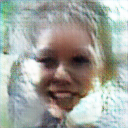
\includegraphics[width=120px]{./photos_from_epoch_8/samples_8_199.png}%
\caption{a man with a beard and a tie is smiling .}%
\end{figure}

%
\end{document}